%%%%%%%%%%%%%%%%%%%%%%%%%%%%%%%%%%%%%%%%%%%%%%%%
% 1: Introducción
%%%%%%%%%%%%%%%%%%%%%%%%%%%%%%%%%%%%%%%%%%%%%%%%
\pagenumbering{arabic} % para empezar la numeración con números
\chapter{Introducción}\label{introduccion}


%Desde el comienzo de su historia, la informática ha intervenido en cada aspecto científico y social existente. La dependencia de la sociedad en una ciencia tan reciente resalta la importancia de que sea algo comprensible y comprendido para la sociedad misma. 

Como dice Maude Lemaire\cite{lemaire2014incorporating}, en una sociedad que está incrementando su dependencia a las nuevas tecnologías\footnote{Aquí, con nuevas tecnologías me refiero a productos y proyectos derivados de la Informática y las \acrfull{TIC} como puede ser los proyectos que detallamos en la sección \ref{estado-arte}.}, es imprescindible que las nuevas generaciones desarrollen la habilidad de pensar de manera crítica sobre tecnología.

El \emph{pensamiento computacional}, como se refiere A. Bundy en \cite{bundy2007computational}, afecta a  investigaciones de casi todas las disciplinas, tanto de ciencias como de humanidades. [...] La informática no solo ha permitido que los investigadores puedan hacerse nuevas preguntas, sino también ha permitido aceptar nuevos tipos de respuesta. Por ejemplo, preguntas que requieren el procesamiento de una gran cantidad de datos.  

Es necesario comprender la informática y desarrollar el \emph{pensamiento computacional}. Se necesitan desarrollar nuevas tecnologías, nuevo \gls{hardware} y \gls{software} que automatice tareas largas, complejas y con una alta cantidad de cómputo. Tareas que no siempre los humanos podemos resolver de manera directa. Para conseguir esto, muchas veces es necesario programar. 

Aprender a programar es mencionado como uno de los 7 grandes retos de la educación informática \cite{mcgettrick2005grand} y diversos estudios \cite{renumol2009classification} muestran que las principales dificultades para un alumno cuando está en el proceso de aprender a programar son (a) como empezar un programa; (b) comprensión de la sintaxis específica del lenguaje de programación; (c) comprensión de la lógica\footnote{En este caso me refiero a lógica booleana, o también llamada Álgebra de Boole.} y (d) problemas a la hora de depurar el código escrito. 

Aunque a primera vista aprender a programar pueda parecer una tarea ardua y compleja, tiene sus ventajas. En el estudio realizado por Janet Siegmund {\color{red}et al} en \cite{siegmund2014understanding}, podemos ver como los participantes mientras comprendían, analizaban y buscaban errores en pequeños trozos de código, daban claras muestras de estar desarrollando actividad cerebral en regiones del cerebro relacionadas con el procesado del lenguaje, la atención y la memoria de trabajo.

De la misma manera, estudios realizados en niños \cite{clements1986effects} de entre 6 y 8 años, muestran que estos demostraron mayor capacidad de atención, más autonomía y un mayor placer por el descubrimiento de nuevos conceptos. En la misma linea, un estudio en niños de infantil \cite{logo-geometry} que utilizaban el \Gls{logo} demostró que los mismos obtuvieron mejores resultados en pruebas de razonamiento, matemáticas o resolución de problemas. Otro estudio más reciernte \cite{liao1991effects} demuestra que aprender a programar (independientemente el lenguaje) potencia la creatividad y la habilidad de aprendizaje en personas de corta edad.



\section{Situación actual}
\label{sub:aprendiendo-programar}


Actualmente existen muchos proyectos para que se introduzca la programación en las aulas y se aprenda a programar desde edades tempranas, ya sea en el aula con un profesor, en casa con los padres o de manera independiente. 


Uno de los proyectos más importantes y con más repercusión a nivel global es Code.org\cite{code-org}. Su proyecto \emph{Hora del código}\cite{hour-of-code} reúne durante una hora al día a decenas de millones de estudiantes de más de 180 países, disponible en más de 30 idiomas. De manera gratuita, cualquiera puede aprender a programar en eventos que se realizan por todo el mundo (figura \ref{fig:map-hour-code}). El proyecto tiene como público objetivo principal a niños de primaria y secundaria. Code.org está apoyado por grandes compañias y persanalidades a nivel global como puede ser Microsoft, Google, el Presidente Barack Obama, Mark Zuckerberg, Bill Gates o Walt Disney Company. {\color{red}En la sección \ref{sec:Code.org} se abordará más detalladamente las diferentes formas que tiene Code.org de enseñar a programar.}


\begin{figure}[!ht]
	\begin{centering}
		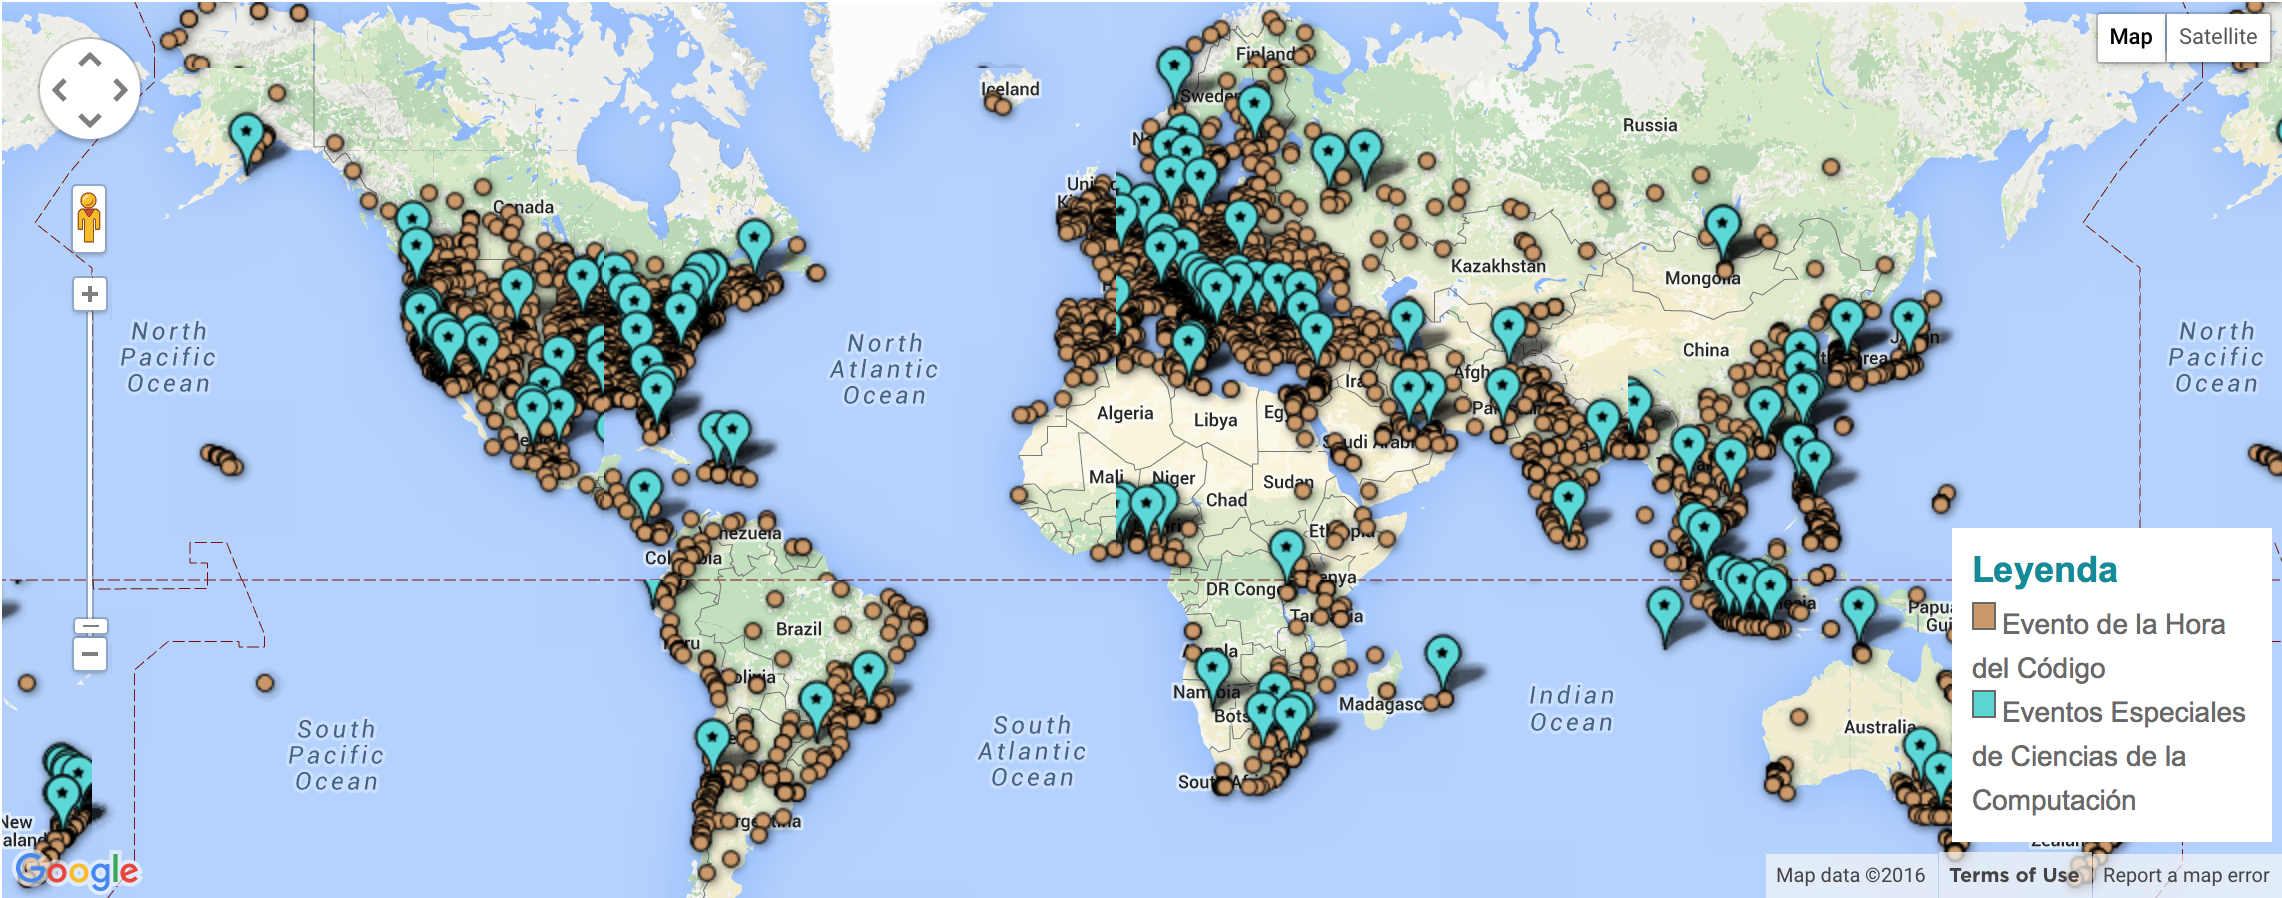
\includegraphics[width=0.8\textwidth]{images/map-hour-code.png}
			\caption{Mapa de visualización de eventos de llevados a cabo por el proyecto \emph{Hora del código} alrededor del mundo. Actualmente 198,473 en todo el mundo, 1,839 en España. Obtenido de \cite{hour-of-code}.}
				\label{fig:map-hour-code}
	\end{centering}
\end{figure}


A nivel europeo, la \Gls{com-euro}{\color{red}\cite{ec-code-week}} ha promovido durante el año 2015 la \emph{EU Code Week}{\color{red}\cite{code-week}} como parte de su Estrategia para la Educación y la Formación 2020. Este proyecto consistió en eventos de una semana de duración en las que se enseñaba informática y programación en lugares de toda Europa\footnote{En España, se realizaron eventos dentro del marco del proyecto \emph{EU Code Week} en Madrid, Sevilla, Murcia, Asturias, Canarias, Cantabria, Zamora, Cataluña, Ceuta, Badajoz, La Rioja, País Vasco y Valencia.}.



\section{Descubre}
\label{sec:descubre}


\section{Motivación y enfoque del proyecto}
\label{sec:motivacion}


%%%%%%%%%%%%%%%%%%%%%%%%%%%%%%%%%%%%%%%%%%%%%%%%
% 2: Estado del arte
%%%%%%%%%%%%%%%%%%%%%%%%%%%%%%%%%%%%%%%%%%%%%%%%
\chapter{Estado del arte}\label{estado-arte}



A nivel global, actualmente existe una gran cantidad de proyectos con la única intención de enseñar, principalmente a algumos de secundaria y bachillerato, diferentes aspectos de la informática como lo es la programación \cite{code-school,code-org,code-academy}, la robótica \cite{robomind-web,moway} e incluso chips y electrónica con \Gls{arduino}\cite{arduino}. Algunos de estos proyectos llevan décadas activos, como lo es el lenguaje \Gls{logo}\cite{logo} y su proyecto \Gls{turtle}\cite{logo-turtle}
La mayoría de estos proyectos promueven una enseñanza independiente y autodidacta bajo un entorno on-line. De esta manera, el alumno puede aprender a su propio ritmo y desde cualquier parte del mundo.


\section{El lenguaje Logo y el robot Turtle}
\label{sec:Logo}

El lenguaje Logo, basado en \Gls{lisp}, fue diseñado como una herramienta para aprendizaje. Todas sus características -interactividad, modularidad, extensibilidad, flexibilidad en los tipos de datos- persiguen esta meta.

%The Logo Programming Language, a dialect of Lisp, was designed as a tool for learning. Its features - interactivity, modularity, extensibility, flexibility of data types - follow from this goal.

Como se explica en la página oficial del proyecto Logo\cite{logo}, durante la década de los 70, en el \acrfull{MIT} y diferentes centros de investigación europeos, se llevó a cabo una investigación sobre el uso del \Gls{logo} en un pequeño grupo de alumnos de secundaria. Todo el proceso se ha documentado en diferentes artículos como \cite{feurzeig1969programming} o \cite{pea1984logo}.

%Throughout the 1970s Logo was incubating at MIT and a few other research sites: Edinburgh, Scotland and Tasmania, Australia. There were small research activities conducted in local schools, including the Brookline Public Schools, just up the Charles River from MIT. Dan Watt, Cynthia Solomon, and other MIT researchers documented their work with a small number of elementary school students using Logo. Their reports are among the several dozen Logo Memos published by MIT during this period.

El proyecto Turtle es el proyecto más popular del lenguaje Logo. Nació como una criatura robótica que se movía por el suelo y se podía programar solo con 2 instrucciones básicas: \texttt{forward x} y \texttt{right y}, para avanzar \texttt{x} \emph{pasos de tortuga} o girar \texttt{y} grados hacia la derecha, respectivamente.

Combinando estas dos instrucciones de lo más simples, nuestro robot tortuga puede realizar cualquier movimiento más complejo, como podemos ver en la figura \ref{fig:mov-tortle}.

\begin{figure}[!ht]
	\begin{centering}
		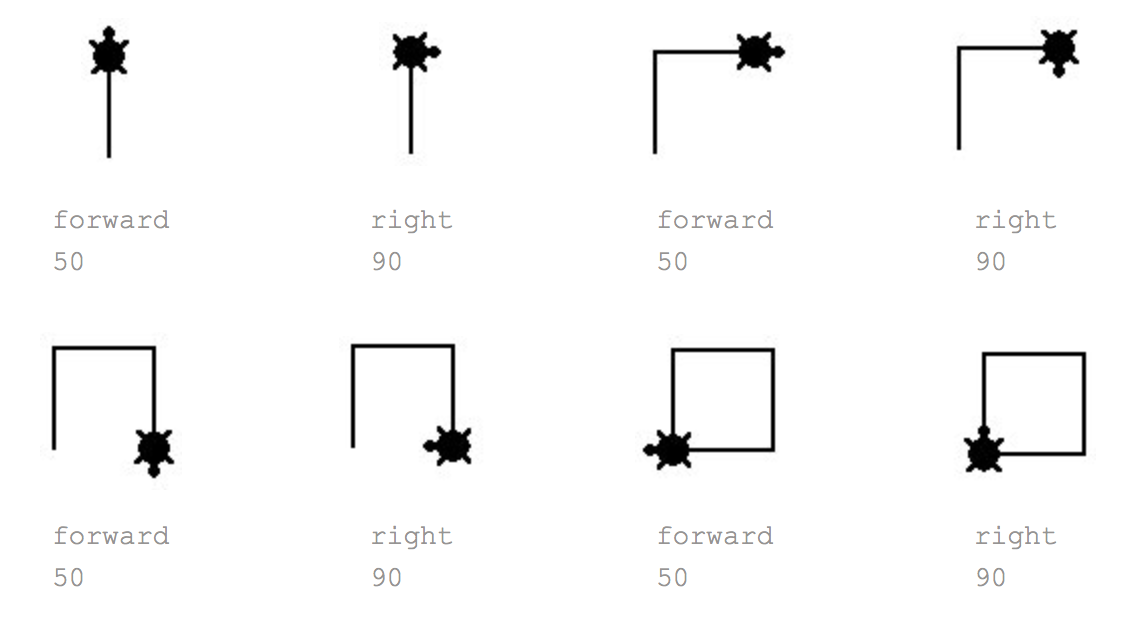
\includegraphics[width=0.8\textwidth]{images/mov-tortle.png}
			\caption{Movimiento de Tortle en forma de cuadrado utilizando unicamente sus instrucciones básicas \texttt{forward} y \texttt{right}.}
				\label{fig:mov-tortle}
	\end{centering}
\end{figure}

Para ilustrar brevemente el lenguaje Logo junto con el robot Turtle, vamos a mostrar como se dibujaría una figura que guarda cierto parecido a una flor.
En el código que se muestra a continuación, creamos una función \texttt{square} que dibuja un cuadrado de tamaño 50 pasos, como podemos ver en la figura \ref{fig:square-turtle}

\begin{lstlisting}
to square
	repeat 4 [forward 50 right 90]
end
\end{lstlisting}

Y a continuación definimos una función \texttt{flower} que utiliza la función \texttt{square} antes descrita y que dibujará una flor, como se puede apreciar en la figura \ref{fig:flower-turtle}

\begin{lstlisting}
to flower
	repeat 36 [right 10 square]
end
\end{lstlisting}

\begin{figure}[!ht]
	\begin{adjustwidth}{\oddsidemargin-1in}{\rightmargin}
	%	\centering
			\begin{subfigure}{\paperwidth}
				\centering
				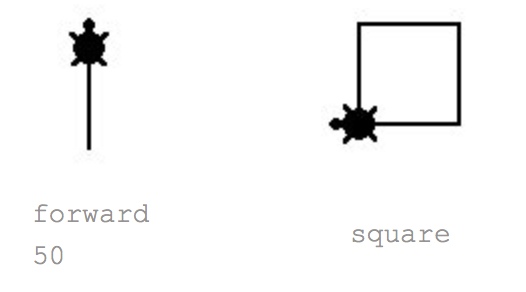
\includegraphics[scale=.45]{images/square-turtle.png}
				\caption{Cuadrado dibujado por el robot Turtle.}
				\label{fig:square-turtle}
			\end{subfigure}
			\begin{subfigure}{\paperwidth}
				\centering
				
\includegraphics[scale=.45]{images/flower-turtle.png}
				\caption{Flor dibujada por el robot Turle.}
				\label{fig:flower-turtle}
			\end{subfigure}
			%\caption{Ejemplo de dibujo utilizando funciones por el robot Turtle.}
		\label{fig:square-flower-turtle}
	\end{adjustwidth}
\end{figure}


El proyecto Tortle ha sido reproducido en proyectos más recientes como \Gls{scratch}\cite{scratch}, el cual se verá en más profundidad en la sección \ref{sec:blockly-scratch}.



\section{Khan Academy}
\label{sec:Khan Academy}

Khan Academy\cite{khan-academy}, con casi 37 millones de usuarios, es uno de los mayores proyectos web para aprender casi de cualquier tema: Matemáticas, estadística, economía o humanidades.


\section{Code.org}
\label{sec:Code.org}

Code.org\cite{code-org} es una plataforma on-line que se dedica exclusivamente a enseñar a programar y cuenta ya con más de 8 millones de usuarios. Cuenta con una gran comunidad de educadores y apoyos entre los que se puede contar al Presidente B. H. Obama. Lleva a cabo proyectos como \emph{Hour of Code} en el que promueve que los usuarios inviertan una hora diaria programando en diferentes juegos, muchos de ellos utilizando \Gls{Blockly}\cite{blockly}.

{\color{red} Parece que estoy haciendo publicidad... shit}


\section{Squeak Etoys}
\label{sec:squeak-etoys}


\section{Blockly y Scratch}
\label{sec:blockly-scratch}


%%%%%%%%%%%%%%%%%%%%%%%%%%%%%%%%%%%%%%%%%%%%%%%%
% 3: Análisis de objetivos y metodología
%%%%%%%%%%%%%%%%%%%%%%%%%%%%%%%%%%%%%%%%%%%%%%%%
\chapter{Análisis de objetivos y metodología}\label{objetivos-metodologia}

\section{Objetivos}
\label{sec:Objetivos}

Este Trabajo Fin de Grado consiste en desarrollar un módulo de simulación de un robot para integrarlo en la plataforma \Gls{descubre}. Para ello se tendrán que cubrir una serie de subobjetivos que nombraremos a continuación.
\begin{itemize}
\item Estudiar el uso y aplicación de diferentes librerías de físicas para generar el robot.
\item Comprensión de la plataforma Descubre así como su posterior modificación.
\item Creación de un simulador de un robot de dos ruedas y su integración en la plataforma Descubre.
\item Modificación del motor de \gls{ijava} y creación de la \acrshort{API} para poder controlar el robot.
\end{itemize}

\section{Metodología}
\label{sec:metodologia}

%%%%%%%%%%%%%%%%%%%%%%%%%%%%%%%%%%%%%%%%%%%%%%%%
% 4: Diseño y resolución del trabajo realizado
%%%%%%%%%%%%%%%%%%%%%%%%%%%%%%%%%%%%%%%%%%%%%%%%
\chapter{Diseño y resolución del trabajo realizado}\label{diseno}




%%%%%%%%%%%%%%%%%%%%%%%%%%%%%%%%%%%%%%%%%%%%%%%%
% 5: Conclusiones y vías futuras
%%%%%%%%%%%%%%%%%%%%%%%%%%%%%%%%%%%%%%%%%%%%%%%%
\chapter{Conclusiones y vías futuras}\label{conslusiones}
